%\titlespacing*{\section}{0pt}{1ex minus 0.2ex}{0.5ex}
\vspace{-2mm}

Our pipeline comprises the following key components: dataset extraction, textual time series annotation, and comprehensive evaluation of the annotations (Figure \ref{fig:flowchart}).

%%%%%%%%%%%%%%%%%%%%%%%%%%%%%%%%%%%%%%%%%%%%%%%%%%%%%
%%%%%%%%%%%%%%%%%%%%%%%%%%%%%%%%%%%%%%%%%%%%%%%%%%%%%
\begin{figure}[tb!]
    \begin{minipage}[t]{0.60\columnwidth}
    \centering
    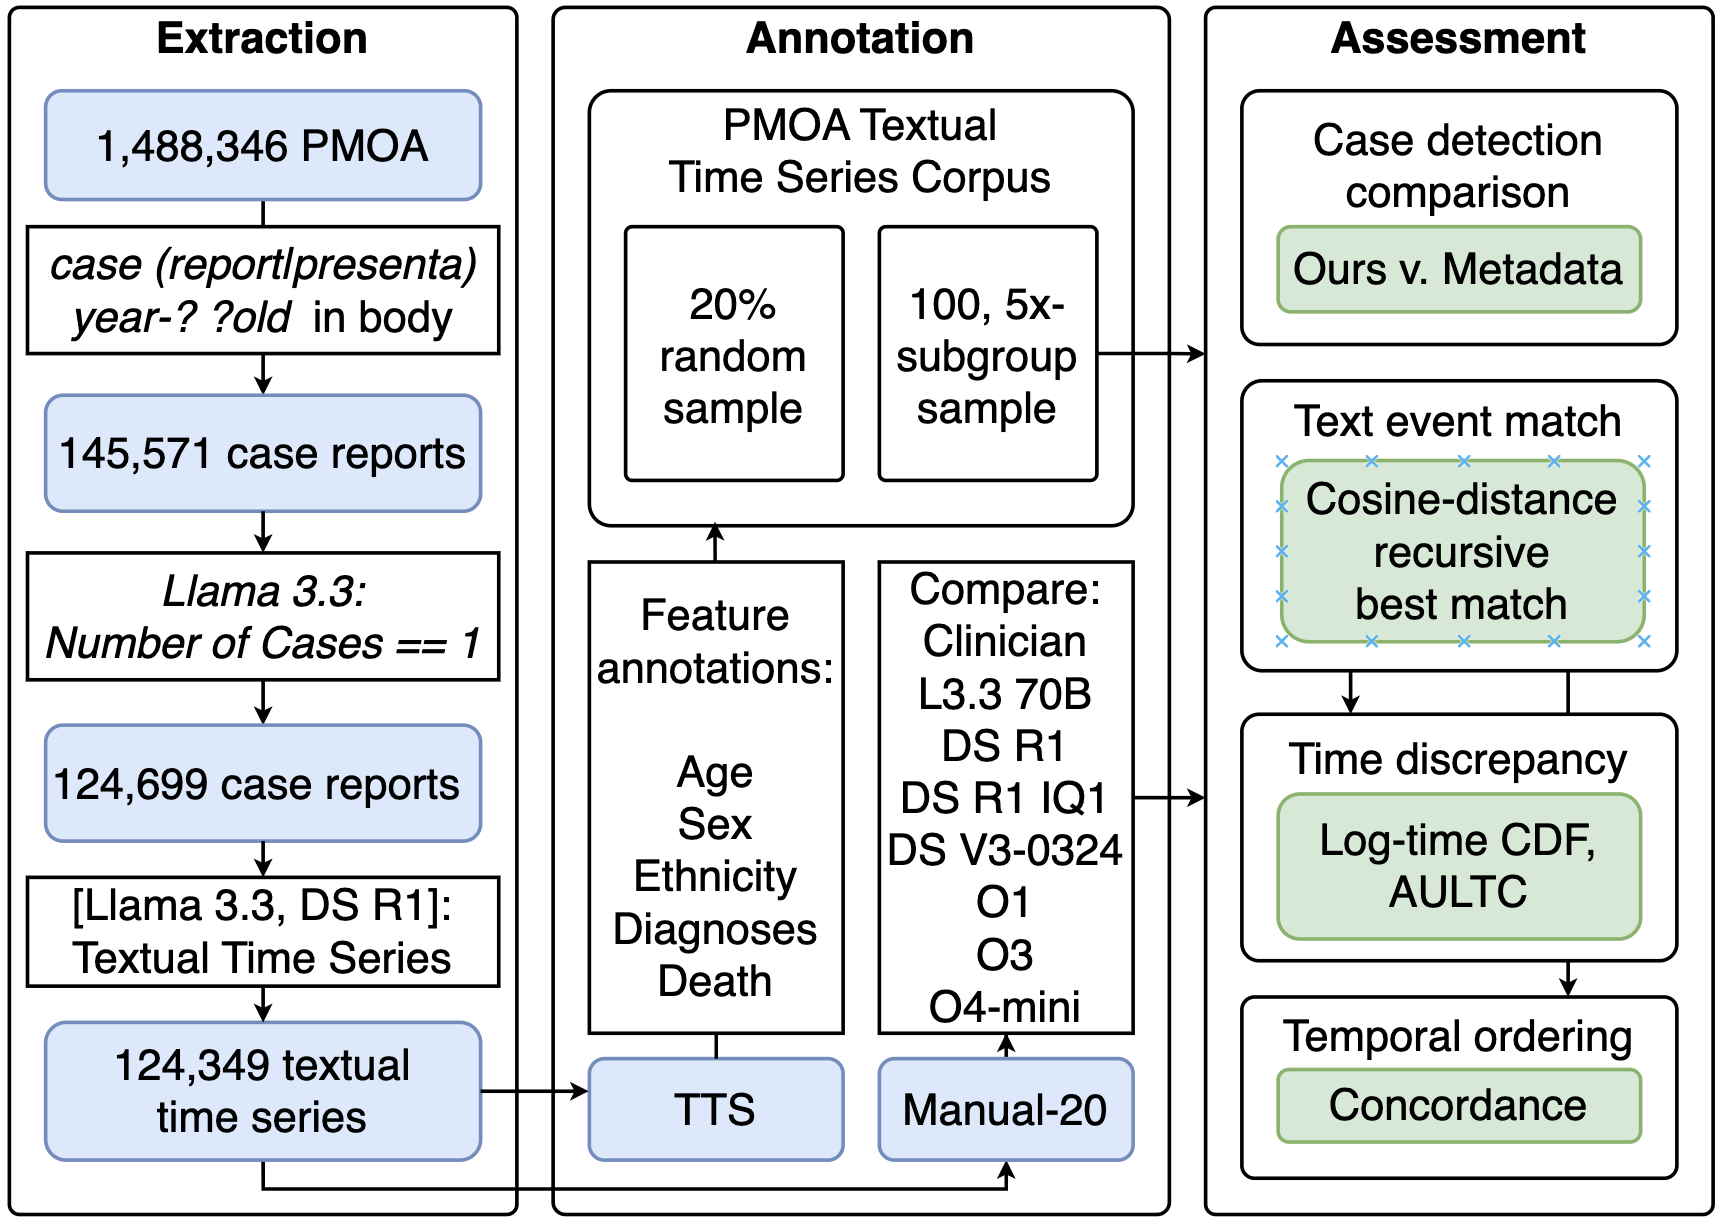
\includegraphics[width=\linewidth]{Plots_tables/PMOATTS_flow4.png}
    \end{minipage}
  %\hfill
  \quad
  \begin{minipage}[t]{0.35\textwidth}
    \vspace{-17.5em}
    \centering
    %%%%%%%% age presentation - top right %%%%%%%%
    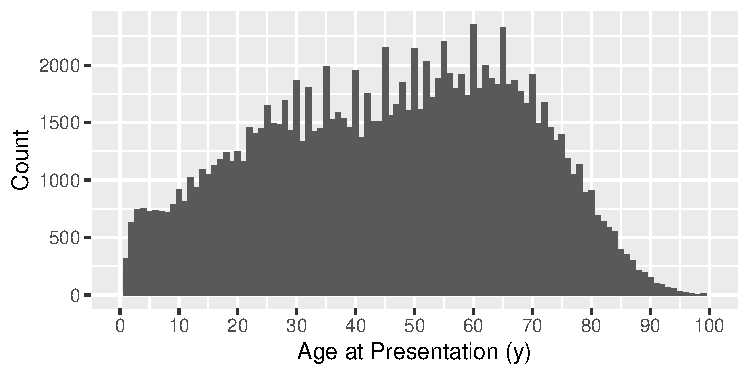
\includegraphics[width=0.87\linewidth]{Plots_tables/125k_age.pdf}
    %\caption{Caption for Figure B.}
    %\label{fig:B}
    \vfill
    \vspace{1em}

    %%%%%%%% demo table - bottom right %%%%%%%%
    \scriptsize
    \begin{tabular}{l r}
    \toprule
    \textbf{Characteristic} & \textbf{Percent (\%)} \\
    \midrule
    \multicolumn{2}{l}{\textbf{Sex}} \\
    \quad Male & 52 \\
    \quad Female & 47 \\
    \quad Not Specified & 1 \\
    \midrule
    \multicolumn{2}{l}{\textbf{Ethnicity}} \\
    \quad White/Caucasian & 5 \\
    \quad Asian & 3 \\
    \quad African & 1 \\
    \quad Other & 2 \\
    \quad Not Specified & 89 \\
    \bottomrule
    \end{tabular}
  \end{minipage}
  \caption{\textbf{Left}: Flowchart of the extraction and annotation pipeline. The left panel (Extraction) shows how we filtered the PMOA corpus to identify single-patient case reports.
  %using heuristic rules and LLM-based classification (LLaMA 3.3 70B Instruct). 
  The middle panel (Annotation) depicts the generation of textual time series for each case via LLM prompting and the creation of evaluation subsets. The right panel (Assessment) summarizes the evaluation process, including metadata comparison, text event matching, time discrepancy analysis (log-time CDF, AULTC), and temporal order concordance. \textbf{Right}: Age, sex, and ethnicity of the PMOA-TTS corpus.}
  \label{fig:flowchart}
  \vspace{-10pt}
\end{figure}
%%%%%%%%%%%%%%%%%%%%%%%%%%%%%%%%%%%%%%%%%%%%%%%%%%%%%%%%
%%%%%%%%%%%%%%%%%%%%%%%%%%%%%%%%%%%%%%%%%%%%%%%%%%%%%%%%

% \begin{figure}[!htbp]
%     \centering
%     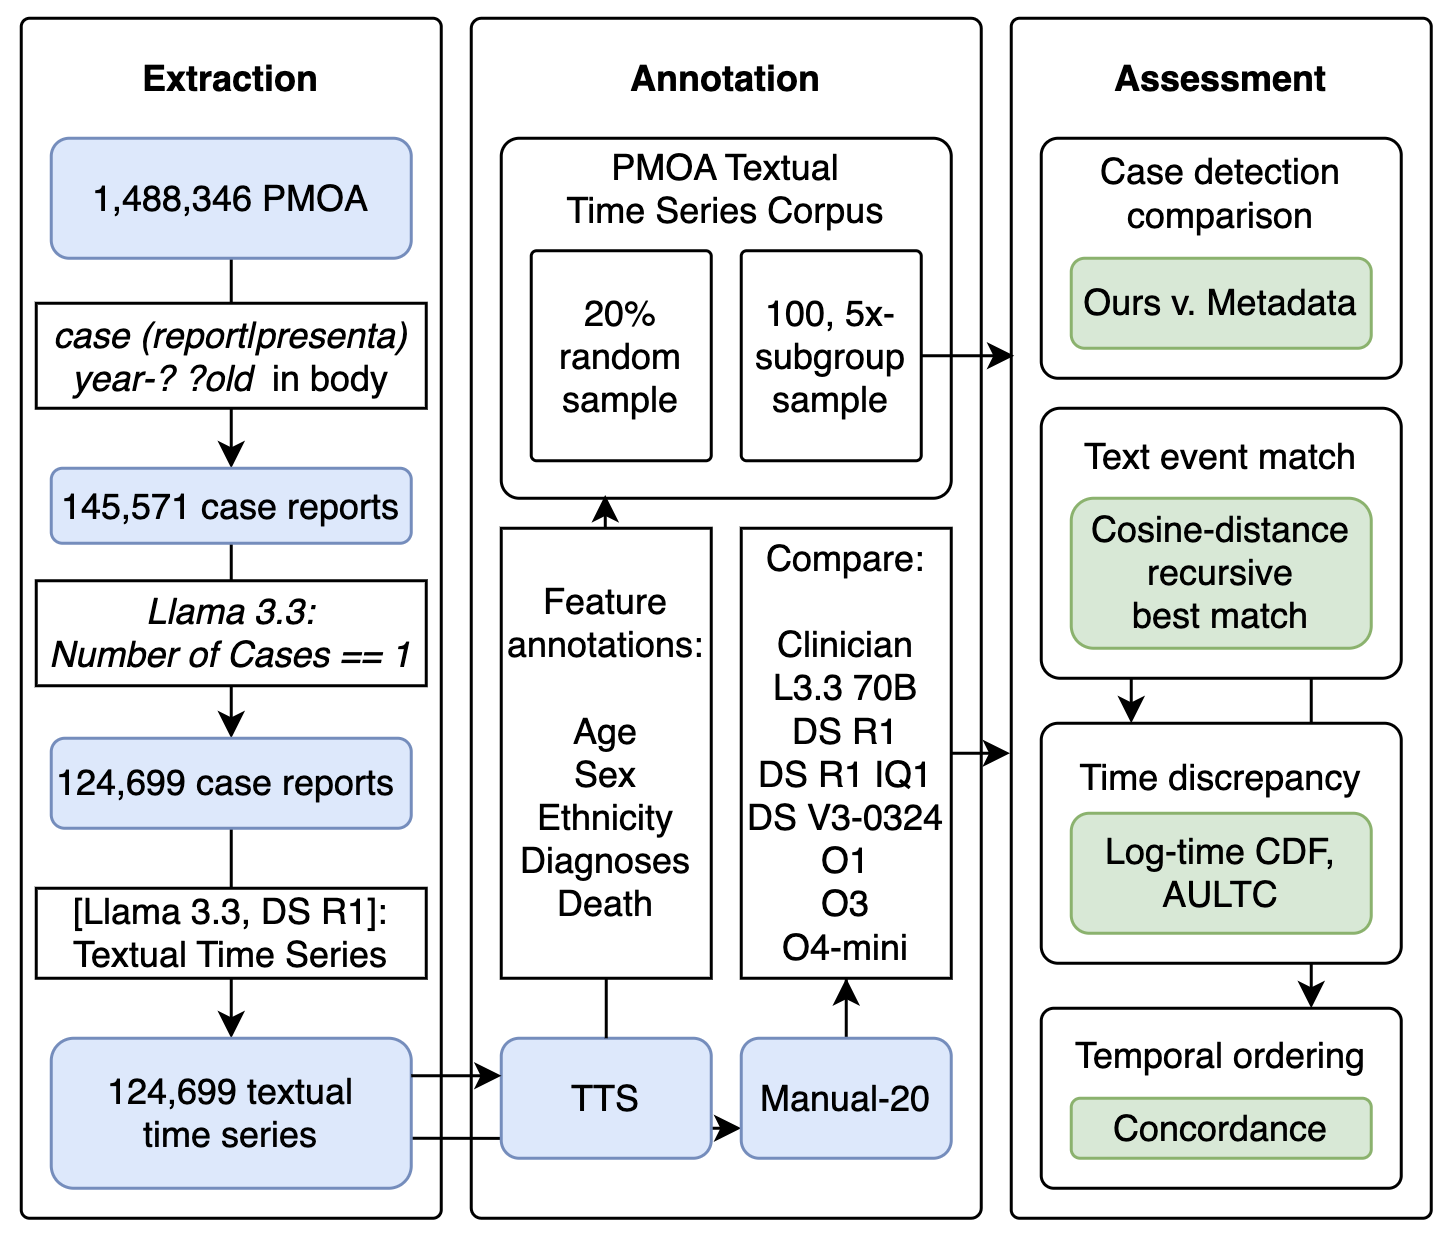
\includegraphics[width=0.62\columnwidth]{Plots_tables/PMOATTS_flow2.png}
%     \caption{Flowchart of the extraction and annotation pipeline. 
%     The left panel (Extraction) shows how we filtered the PMOA corpus to single-patient case reports using heuristic search and LLM-based classification (LLaMA 3.3 70B). 
%     The middle panel (Annotation) illustrates the creation of the textual time series for each case report using LLM prompting, as well as the generation of evaluation subsets. 
%     The right panel (Assessment) outlines evaluation steps including comparison to metadata-based identification, text event matching metrics, time discrepancy analysis (log-time CDF and AULTC), and temporal order concordance.}
%     \label{fig:flowchart}
% \end{figure}

\subsection{Case Report Identification Pipeline}

We use the PubMed Open Access (PMOA) repository data, which includes 1.4 million published manuscripts. Specifically, we utilize the plain text files from the December 17, 2024 release, located in the \texttt{oa\_noncomm} folder, which supports both noncommercial and commercial use. Following the method in \cite{wang2025large}, we identify candidate case reports by extracting content between the section markers ``\texttt{==== Body}'' and ``\texttt{==== Ref}'', which separate the main text and references in the PMOA format.

To ensure relevance, we first filter documents by matching the body text with the regular expressions ``\texttt{(case report|case presenta)}'' and ``\texttt{year-? ?old}''. This filter yields 145,571 candidate documents likely to be case reports or case series. To narrow this set to single-patient case reports, we use a large language model (LLaMA 3.3 70B Instruct) to analyze each document's body text. The model is prompted with: ``\texttt{You are a physician. Determine the number of case reports in the following manuscript. Return 0 if it is not a case report. Reply only with the number and nothing else.}'', followed by the document body. We retain documents for which the model replies with \texttt{1} and discard others. This two-stage process results in a final dataset of 124,699 single-patient case reports (Figure~\ref{fig:flowchart}).

We compared our LLM-based case report identification method with PubMed's metadata-based labeling using a carefully designed benchmark. We created a dataset of 100 reports across five diagnoses—Diabetes, Sepsis, Hypertension, COVID-19, and Atrial Fibrillation—with 10 reports per diagnosis from each method. A clinician manually reviewed and labeled each report to verify whether it described exactly one case. Our LLM-pipeline significantly outperforms PubMed metadata filtering, particularly in terms of specificity and precision (Section~\ref{sec:results_case_identification}).


% \begin{figure}[!htbp]
%     \centering
%     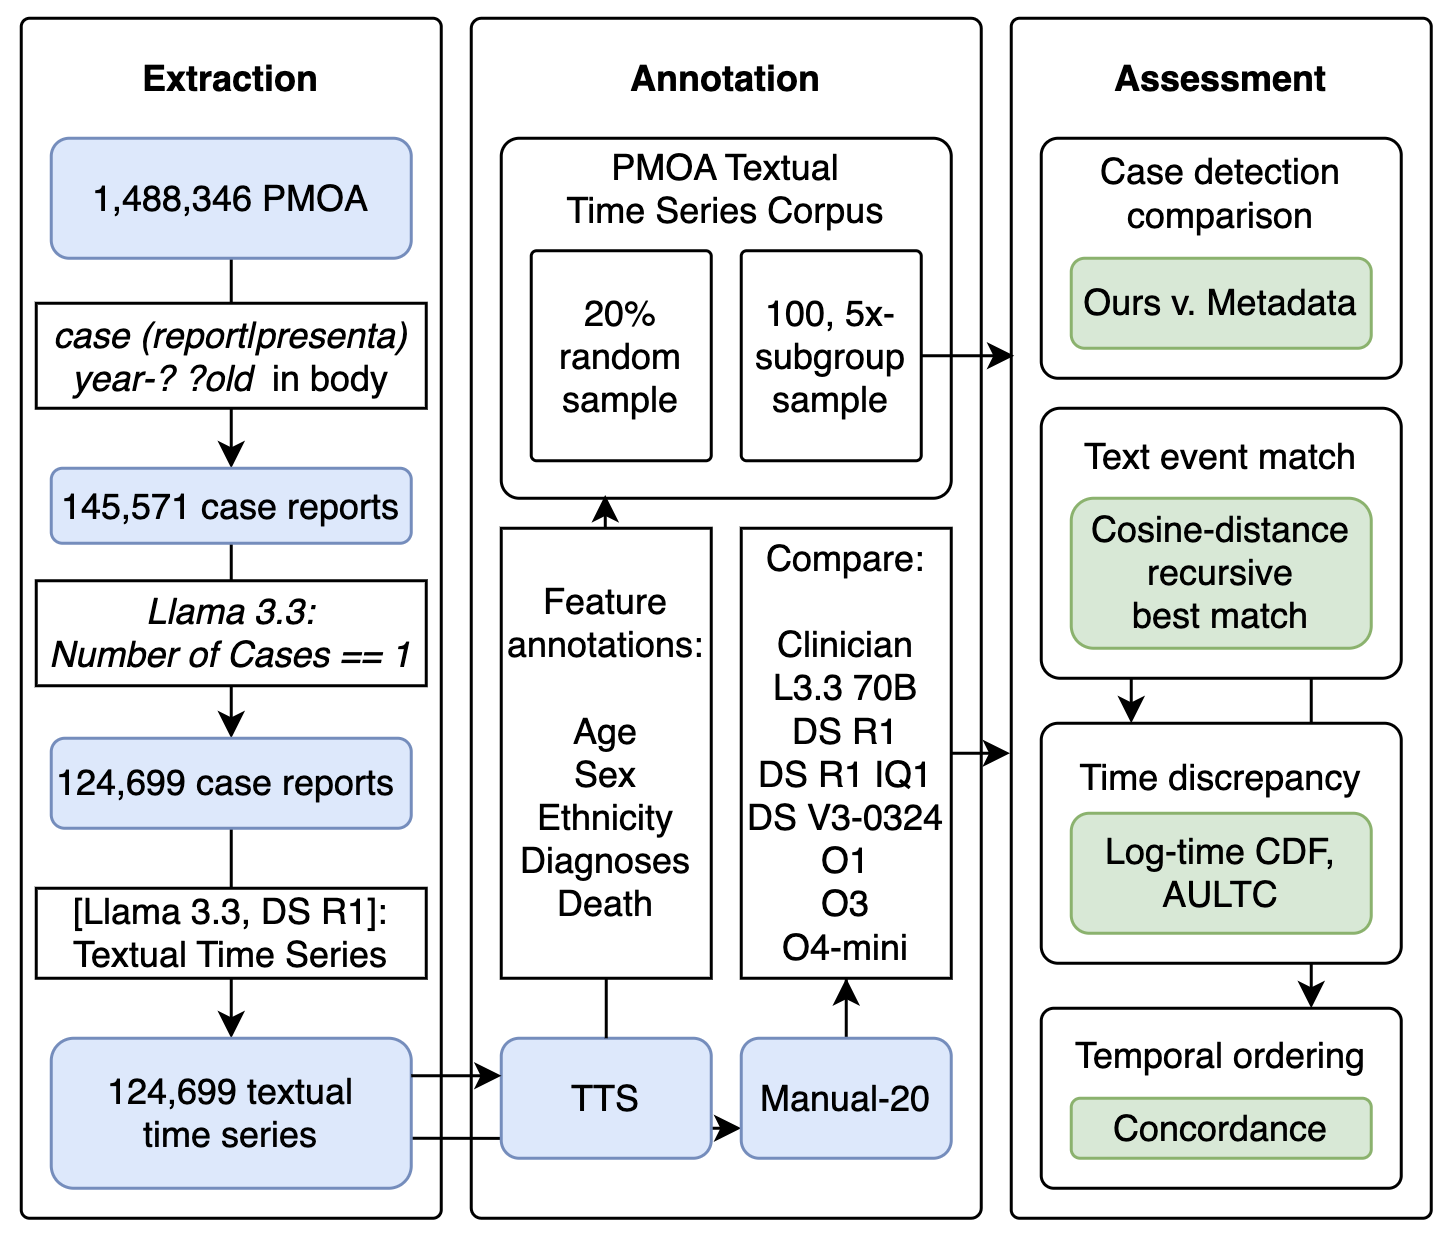
\includegraphics[width=0.62\columnwidth]{Plots_tables/PMOATTS_flow2.png}
%     \caption{Flowchart of the extraction and annotation pipeline. 
%     The left panel (Extraction) shows how we filtered the PMOA corpus to single-patient case reports using heuristic search and LLM-based classification (LLaMA 3.3 70B). 
%     The middle panel (Annotation) illustrates the creation of the textual time series for each case report using LLM prompting, as well as the generation of evaluation subsets. 
%     The right panel (Assessment) outlines evaluation steps including comparison to metadata-based identification, text event matching metrics, time discrepancy analysis (log-time CDF and AULTC), and temporal order concordance.}
%     \label{fig:flowchart}
% \end{figure}


% We note that this identification process, while high throughput, still carries some noise due to LLM errors. 
% We compared our LLM-based identification to the PubMed metadata labeling. 
% A manual review of a small random sample (N=100) from the final set confirmed a >95\% precision for true single-patient case reports, with a few borderline cases (e.g., case series of two patients) incorrectly included. 
% Overall, the two-stage approach provides a scalable and accurate solution to compile the corpus.

\subsection{Timeline Annotation via LLM Prompting}
We used LLMs to extract clinical textual time series from PMOA case reports. A textual time series is a chronologically ordered sequence of clinical findings, each associated with a timestamp and a specific patient. A clinical finding refers to a free-text description of a health-related condition affecting the patient. Our approach differs from conventional methods (e.g., \cite{sun2013evaluating, uzuner20112010}) by capturing longer, more context-rich text spans to accurately convey the meaning of clinical findings. Unlike the i2b2 guidelines, we do not limit findings to short prepositional phrases. For example, ``pain in chest that radiates substernally'' is kept intact to preserve its clinical nuance. Additionally, coordinated findings are separated for clarity—e.g., ``metastases in the liver and pancreas'' is split into ``metastasis in the liver'' and ``metastasis in the pancreas.''

To construct clinical textual time series, we adopt the LLM extraction prompt from previous work \citep{wang2025large,noroozizadeh2025reconstructing}. This prompt instructs the LLM to extract clinical events with timestamps, setting the admission event at a reference time of 0, with other events expressed in relative hours (negative for pre-admission events, positive for post-admission). It also provides guidelines for handling conjunctions, event durations, and output formatting (full prompt in Appendix \ref{apd:extraction_prompt}).

For each report, the LLM generates a structured sequence of (clinical\_event, time) tuples. Events are retained in free-text form to preserve their clinical specificity, rather than being mapped to a fixed ontology. On average, each report contains 46 events, with significant variation depending on report length and complexity. The corpus as a whole includes over 5.6 million temporally anchored events, making it one of the largest datasets of its kind in clinical NLP.
Computational resources used are described in Appendix \ref{apd:compute_resources}.


%%%%%%%%%%%%%%%%%%%%%%%%%%%%%%%%%%%
%%%%%%%%%%%%%%%%%%%%%%%%%%%%%%%%%%
% \subsection{Diagnosis and Demographic Extraction}

% In addition to timeline extraction, we used tailored LLM prompts to extract both diagnoses and demographic information from the case reports.

% For diagnosis extraction, the LLM was prompted to act as an expert physician and return a list of patient-specific diagnoses from the report, clearly distinguishing true diagnoses (e.g., “acne,” “DRESS syndrome”) from general clinical findings (e.g., “rash,” “leukocytosis”). The prompt directed the model to list the primary diagnosis first, include one diagnosis per line, and omit any explanatory text (full prompt in Appendix \ref{apd:diagnosis_prompt}).

% For demographic extraction, we applied an LLM-based query to retrieve age, sex, and ethnicity. The prompt specified that age be reported in years, sex as Male, Female, a custom string, or Not Specified, and ethnicity in accordance with U.S. Census categories or as Not Specified (see Appendix \ref{apd:demographics_prompt}). This enabled us to characterize the demographic composition of the corpus population, as described in Section \ref{sec:demographics}.


\subsection{Manual Annotations for Evaluation}

We combined manual annotations from \cite{wang2025large} and \cite{noroozizadeh2025reconstructing} to serve as ground truth for evaluating the quality of LLM annotations. 
The manual annotation process was conducted by expert physicians and followed the ISO-TimeML specification, which includes actions or states inferred to have occurred or held true. 
Annotators selected exact text spans representing events, with two exceptions to enhance usability: (i) conjunctive lists could be split into individual events, and (ii) the prefix ``history of'' could be added when contextually appropriate. 
These adjustments preserved the original text alignment for downstream analysis. 
Each event was then assigned a time relative to the case reference point (e.g., admission or encounter date), using the start time when an interval was described.

This manually annotated subset of 20 cases serves as the gold standard for our evaluation metrics, described in the following section.


\subsection{Evaluation Metrics}

We assessed the textual time series extracted from PMOA case reports using three key metrics: event match rate, temporal concordance (c-index), and log-time discrepancy.

%\subsubsection{Text Event Match}

\textbf{Text Event Match.} To evaluate the alignment between predicted clinical findings and reference annotations, we used a recursive best-match strategy \citep{wang2025large, noroozizadeh2025reconstructing}. This method pairs events by minimizing string-based distances while avoiding many-to-one mappings. For each reference event, the closest predicted event is selected based on the minimal distance, with event order used to break ties. Once matched, both events are removed from further consideration, and the process continues recursively with the remaining pairs.

We tested several distance metrics, including Levenshtein distance, cosine similarity of BERT (bert-base-uncased) embeddings, and cosine similarity based on sentence embeddings from PubMedBERT (S-PubMedBert-MS-MARCO). Previous validation showed that PubMedBERT-based cosine similarity with a threshold of 0.1 was the most reliable, and we used this metric for our evaluation. A detailed description of the algorithm is provided in Appendix \ref{apd:recursive_match}.

%\subsubsection{Temporal Ordering}

\textbf{Temporal Ordering.} To quantify the accuracy of temporal ordering, we used the concordance index (c-index), which measures the probability that a randomly selected pair of predicted findings is correctly ordered in time. Higher c-index values indicate better alignment with the reference timeline. Formally, for a set of events with reference times $\{t^r_i\}$ and predicted times $\{t^p_i\}$, the c-index is calculated as $\text{c-index} = \frac{1}{N} \sum_{i<j} \mathds{1}\{(t^r_i - t^r_j)(t^p_i - t^p_j) > 0\}$ where $N$ is the number of comparable pairs (event indices $i, j$ such that $t^r_i \neq t^r_j$ and $t^p_i \neq t^p_j$), and $\mathds{1}\{\cdot\}$ is the indicator function.

% \vspace{-10pt}
% \begin{equation}
% \text{c-index} = \frac{1}{N} \sum_{i<j} \mathbf{1}[(t^r_i - t^r_j)(t^p_i - t^p_j) > 0]
% \end{equation}
% \vspace{-10pt}

%\subsubsection{Time Discrepancy Analysis}

\textbf{Time Discrepancy Analysis.} We evaluated temporal prediction accuracy by measuring the discrepancies between predicted and reference timestamps. Log-time discrepancy was computed as $\log(1 + \Delta t)$, where $\Delta t$ is the absolute time difference (in hours). To summarize these discrepancies, we introduced the Area Under the Log-Time Cumulative Distribution Function (AULTC), which quantifies how quickly the cumulative distribution of time errors rises—higher AULTC values indicate better temporal alignment. The full definition of AULTC is in Appendix \ref{apd:ltcdf}. We also stratified the analysis by reference time intervals (hour, day, week, year) to examine how prediction accuracy varies with time from case presentation.

\subsection{Downstream Applications}

To demonstrate the utility of the PMOA-TTS corpus for clinical prediction tasks, we implemented two downstream applications: survival analysis and event forecasting.

\textbf{Survival Analysis.}
An example downstream task enabled by PMOA-TTS is survival analysis, where the objective is to predict time until death extracted from each case report. 
We adopt a two-stage framework: first, each textual timeline is converted into a structured context of timestamped clinical events (following the Triplet encoding approach in \cite{oufattolemeds}) and embedded using various pre-trained encoder and decoder language models. 
For encoder models, we extract the \texttt{[CLS]} token embedding; for decoder models, we compute the mean over non-padding token embeddings. Second, these representations serve as covariates for two survival models: DeepSurv \citep{katzman2018deepsurv} and DeepHit \citep{lee2018deephit}. 
Performance is evaluated using the time-dependent concordance index \citep{antolini2005time} and the integrated Brier score, with hyperparameter tuning on a validation set and final evaluation on a held-out test set. 
To ensure robustness, experiments were repeated across five random seeds. Full experimental details are provided in Appendix~\ref{apd:survival_analysis}.

\textbf{Event Forecasting Applications.}
In parallel work by \cite{noroozizadeh2025forecasting}, the utility of textual time series for forecasting tasks has been demonstrated on a smaller cohort of sepsis patients. 
That work formulated two specific forecasting tasks: 

1. \emph{Next Event Timing (F1)}: Given a history of (clinical\_event, time) tuples, predicting whether the next \(k\) events will occur within specific time windows (1 hour, 1 day, 1 week).

2. \emph{Event Ordering (Concordance)}: Given a history of (clinical\_event, time) tuples, predicting the correct temporal ordering of the next \(k\) events.

A summary of these forecasting tasks and their experimental results from the PMOA-TTS subset used in \cite{noroozizadeh2025forecasting} are provided in Appendix~\ref{apd:forecasting} for completeness.

% Our findings revealed that off-the-shelf LLMs face significant challenges when performing forecasting tasks on the textual time series data, highlighting the need for more specialized methodological development in this area. 
% This opens an important avenue for future research, where our expanded PMOA-TTS corpus could serve as a valuable resource for developing and evaluating improved forecasting approaches across a broader range of clinical conditions.
% A summary of these experiments are provided in Appendix~\ref{apd:forecasting}.





%%% Duplicate
% \subsection{Demographic sample}
% We selected a random 20\% case report sample to better characterize our population.  
% We used LLM-based queries to extract the age, sex and ethnicity of our population.
% In contrast to the demographic characterization in \cite{zhao2023large}, our sample is only among single-case case reports, which contain more detailed content than the multi-case reports.  
% Additionally, our extraction uses prompts rather than regular expressions, and we also request recovery of ethnicity according to the United States Census groups (Prompt in Appendix \ref{apd:demographics_prompt}).

%%%%%%%%%%%%%%%%%%%%%%%%%%%%%%%%%%%%%%%%%%%%%%%%%%%%%%%%%%%%
%%%%%%%%%%%%%%%%%%%%%%%%%%%%%%%%%%%%%%%%%%%%%%%%%%%%%%%%%%%%
%%%%%%%%%%%%%%%%%%%%%%%%%%%%%%%%%%%%%%%%%%%%%%%%%%%%%%%%%%%%

% % DEMOGRAPHICS
% % # In 10.000 sample,
% % # 52 % male, 47 % female, 1% not specified
% % # US Census ethnicity
% % #   89 % Not Specified
% % #    5 % White/Caucasian
% % #    3 % Asian
% % #    1 % African
% % #    2 % Other
% \noindent
% \begin{minipage}[t]{\textwidth}
%     \begin{minipage}[t]{0.48\columnwidth}
%         \centering
%         % \begin{figure}[htb]
%         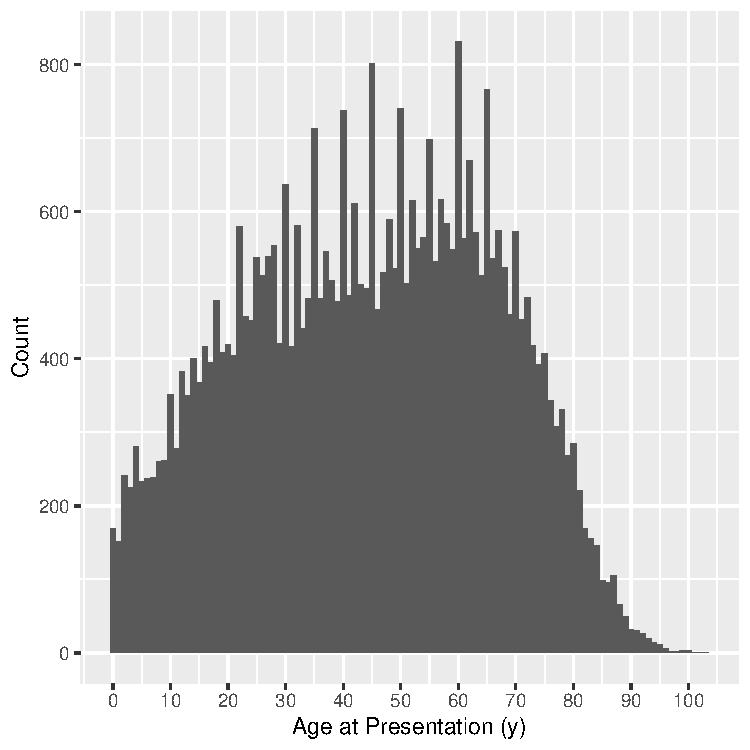
\includegraphics[width=\columnwidth]{Plots_tables/25k_age.pdf}
%         % \captionof{figure}{Histogram of Age (years) in the PMOA 20\% sample.}
%         % \label{fig:age}
%         % \end{figure}
%     \end{minipage}
%     \hfill
%     \begin{minipage}[t]{0.48\columnwidth}
%         \vspace*{-18em}
%         \centering
%         % \begin{table}[h]
% \caption{Demographic characteristics of the PMOA 10,000 sample}
% \captionof{table}{Demographic characteristics of the PMOA 10,000 sample}
% \label{tab:demographics}
\vspace{0.5em}
\centering
\begin{tabular}{l r}
\toprule
\textbf{Characteristic} & \textbf{Percent (\%)} \\
\midrule
\multicolumn{2}{l}{\textbf{Sex}} \\
\quad Male & 52 \\
\quad Female & 47 \\
\quad Not Specified & 1 \\
\midrule
\multicolumn{2}{l}{\textbf{Ethnicity}} \\
\quad White/Caucasian & 5 \\
\quad Asian & 3 \\
\quad African & 1 \\
\quad Other & 2 \\
\quad Not Specified & 89 \\
\bottomrule
\end{tabular}
% \end{table}
%     \end{minipage}
%     \captionof{figure}{Age, sex, and ethnicity of the PMOA 20\% random sample.}
%     \label{fig:demographics}
% \end{minipage}

%--------------------------------------
% \subsection{Diagnosis}